\documentclass{beamer}
\usepackage{graphicx}
\usepackage{subfigure}
\usepackage{caption}
\usepackage{color}
\usepackage{hyperref}
% NOTE: If you want to change the layout, have a look at:
%       http://www.hartwork.org/beamer-theme-matrix/
%       The nice thing about Goettingen (and some other themes)
%       is the outline you get for free (at the right side).
%       Of course, you can also change every aspect of the layout,
%       or even define your own layout, if you want!
\usetheme{Goettingen}     % row name
\usecolortheme{seahorse}  % column name

\mode<presentation>

\title{Structure from Visibility: \\
       Finding low-textured and reflective occluders in outdoor scenes
       using visibility and occlusion}
\author[Martijn van der Veen]{Martijn van der Veen}
\date[10-09-2012]{September 10, 2012}

\begin{document}


\begin{frame}
  \titlepage
  \begin{center}
    Supervisor: Gabriel J. Brostow
  \end{center}
\end{frame}

\section{Introduction}

\begin{frame}
  \frametitle{Outline}
  \setcounter{tocdepth}{1}
  \tableofcontents % <- NOTE: will generate automatically based on section and subsection titles
                   %          (i didn't want the subsection titles, so did it by hand)
\end{frame}

\begin{frame}
  \frametitle{Introduction}
  Goal: reconstructing (difficult) objects in outdoor scenes \\ using a set of images
  \begin{figure}[htb!]
   \centering
   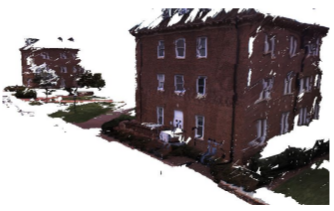
\includegraphics[width=0.6\textwidth]{img/3dmodel}
   \caption*{\tiny Source: P. Merrell et al. [2007]} % cheating a bit with depth map results :-)
   \label{fig:3dmodel}
  \end{figure}
\end{frame}


\section{Previous Work}

\begin{frame}
  \frametitle{Previous Work}
  \begin{itemize}
    \item Structure from Motion (sparse point clouds)
    \item Space Carving using Silhouettes
    \item Multi-View Stereo (Depth Maps)   % dense point cloud
  \end{itemize}
\end{frame}


\subsection{Structure fr. Motion}

\begin{frame}
  \frametitle{Structure from Motion}
  \begin{itemize}
    \item Find and Match interesting points
    \item Estimate camera positions
    \item Triangulate point locations
    \item Make visibility lists
  \end{itemize}
  \begin{figure}[htb!]
   \centering
   \includegraphics[width=0.7\textwidth]{img/sfm1}
  \end{figure}
\end{frame}

\begin{frame}
  \frametitle{Structure from Motion}
  \begin{itemize}
    \item \textbf{Find and Match interesting points}
    \item Estimate camera positions
    \item Triangulate point locations
    \item Make visibility lists
  \end{itemize}
  \begin{figure}[htb!]
   \centering
   \includegraphics[width=0.7\textwidth]{img/sfm2}
  \end{figure}
\end{frame}

\begin{frame}
  \frametitle{Structure from Motion}
  \begin{itemize}
    \item Find and Match interesting points
    \item \textbf{Estimate camera positions}
    \item Triangulate point locations
    \item Make visibility lists
  \end{itemize}
  \begin{figure}[htb!]
   \centering
   \includegraphics[width=0.7\textwidth]{img/sfm3}
  \end{figure}
\end{frame}

\begin{frame}
  \frametitle{Structure from Motion}
  \begin{itemize}
    \item Find and Match interesting points
    \item Estimate camera positions
    \item \textbf{Triangulate point locations}
    \item Make visibility lists
  \end{itemize}
  \begin{figure}[htb!]
   \centering
   \includegraphics[width=0.7\textwidth]{img/sfm4}
  \end{figure}
\end{frame}

\begin{frame}
  \frametitle{Structure from Motion}
  \begin{itemize}
    \item Find and Match interesting points
    \item Estimate camera positions
    \item Triangulate point locations
    \item \textbf{Make visibility lists}
  \end{itemize}
  \begin{figure}[htb!]
   \centering
   \includegraphics[width=0.7\textwidth]{img/sfm5}
  \end{figure}
\end{frame}

\begin{frame}
  \frametitle{Structure from Motion}
  We get:
  \begin{itemize}
    \item \textbf{Sparse} Point Cloud
    \item Camera models (poses, etc)
    \item Visibility lists
  \end{itemize}
  \begin{figure}[htb!]
   \centering
   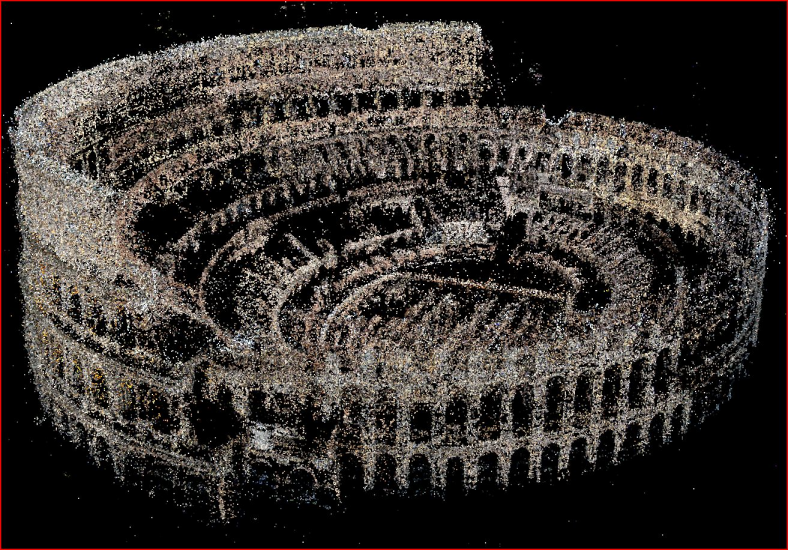
\includegraphics[width=0.8\textwidth]{img/sfm_sparsepointcloud}
  \end{figure}
\end{frame}


\subsection{Space Carving}

\begin{frame}
  \frametitle{Space Carving (silhouettes)}
  \begin{figure}[htb!]
   \centering
   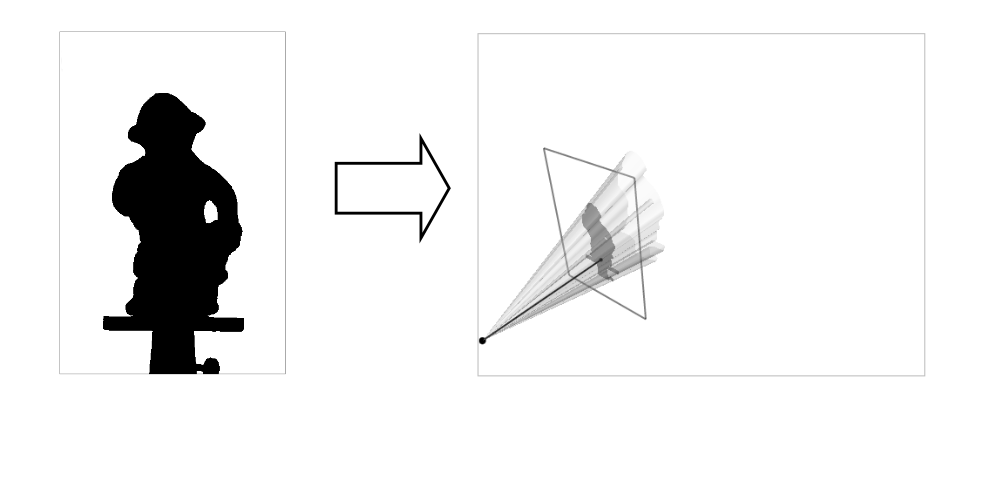
\includegraphics[width=1.0\textwidth]{img/carving1}
   \caption*{\tiny Source: How to prepare and deliver a presentation, by Roberto Cipolla [ppt]}
   \label{fig:carving1}
  \end{figure}
\end{frame}
\begin{frame}
  \frametitle{Space Carving (silhouettes)}
  \begin{figure}[htb!]
   \centering
   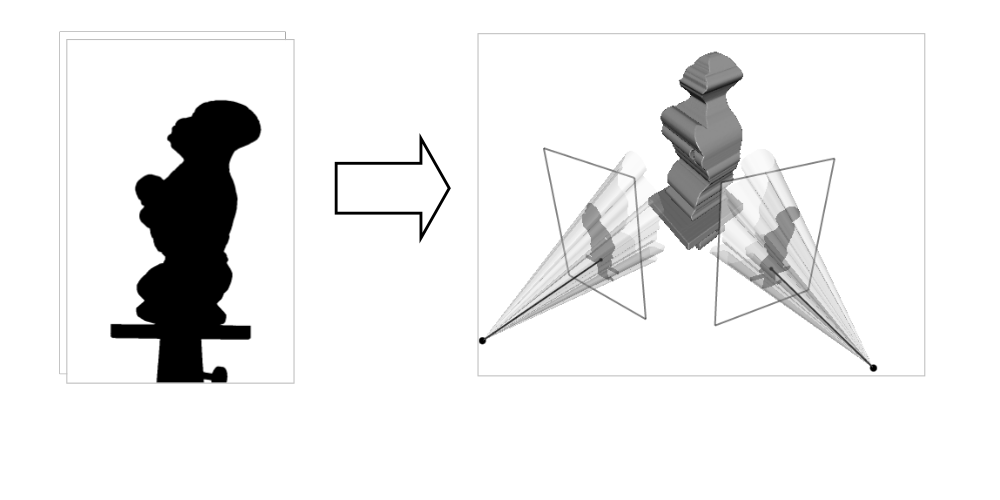
\includegraphics[width=1.0\textwidth]{img/carving2}
   \caption*{\tiny Source: How to prepare and deliver a presentation, by Roberto Cipolla [ppt]}
   \label{fig:carving2}
  \end{figure}
\end{frame}
\begin{frame}
  \frametitle{Space Carving (silhouettes)}
  \begin{figure}[htb!]
   \centering
   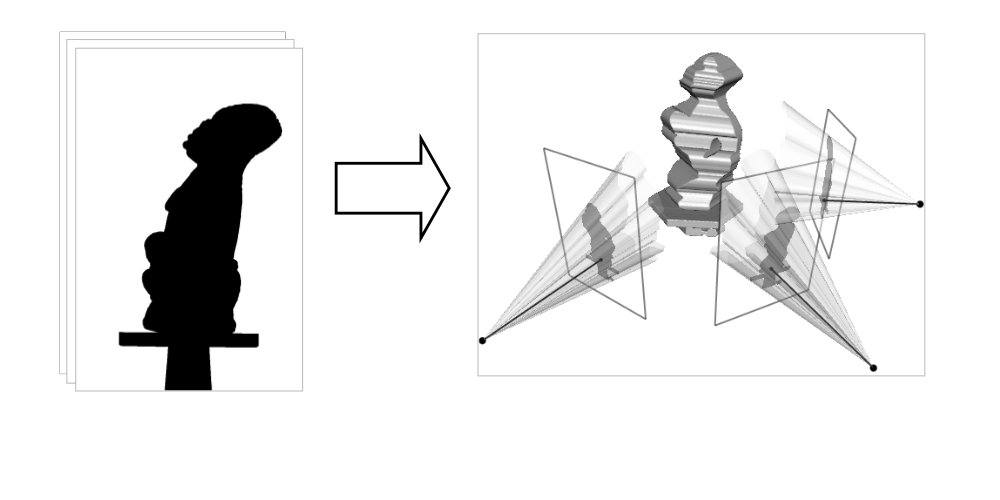
\includegraphics[width=1.0\textwidth]{img/carving3}
   \caption*{\tiny Source: How to prepare and deliver a presentation, by Roberto Cipolla [ppt]}
   \label{fig:carving3}
  \end{figure}
\end{frame}
\begin{frame}
  \frametitle{Space Carving (silhouettes)}
  \begin{figure}[htb!]
   \centering
   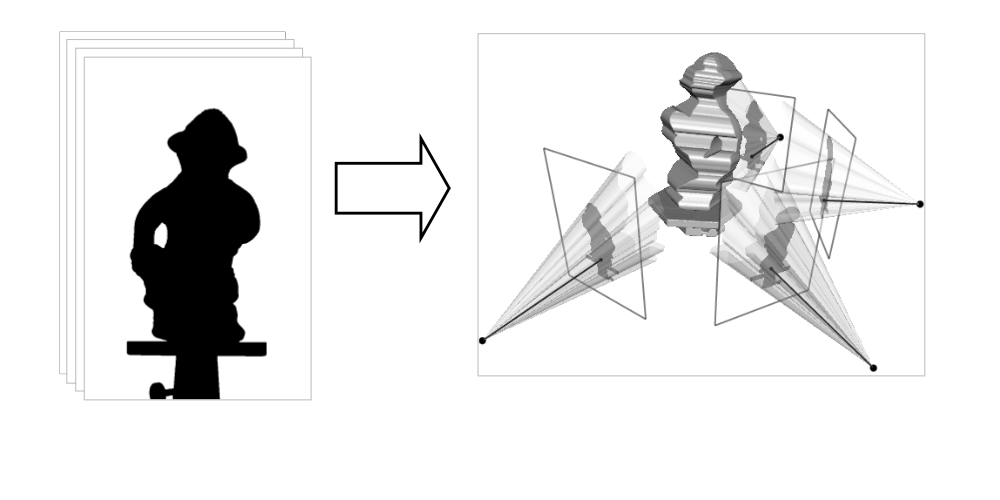
\includegraphics[width=1.0\textwidth]{img/carving4}
   \caption*{\tiny Source: How to prepare and deliver a presentation, by Roberto Cipolla [ppt]}
   \label{fig:carving4}
  \end{figure}
\end{frame}
\begin{frame}
  \frametitle{Space Carving (silhouettes)}
  \begin{figure}[htb!]
   \centering
   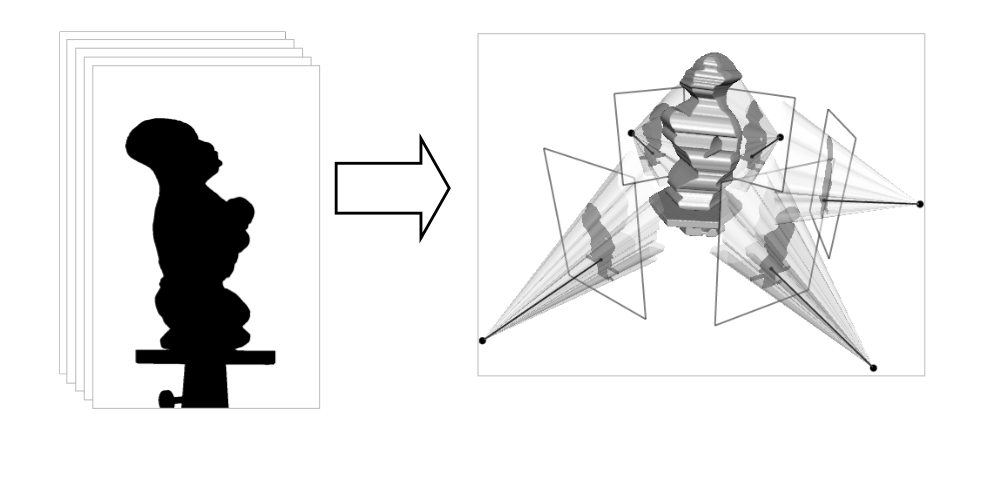
\includegraphics[width=1.0\textwidth]{img/carving5}
   \caption*{\tiny Source: How to prepare and deliver a presentation, by Roberto Cipolla [ppt]}
   \label{fig:carving5}
  \end{figure}
\end{frame}
\begin{frame}
  \frametitle{Space Carving (silhouettes)}
  \begin{figure}[htb!]
   \centering
   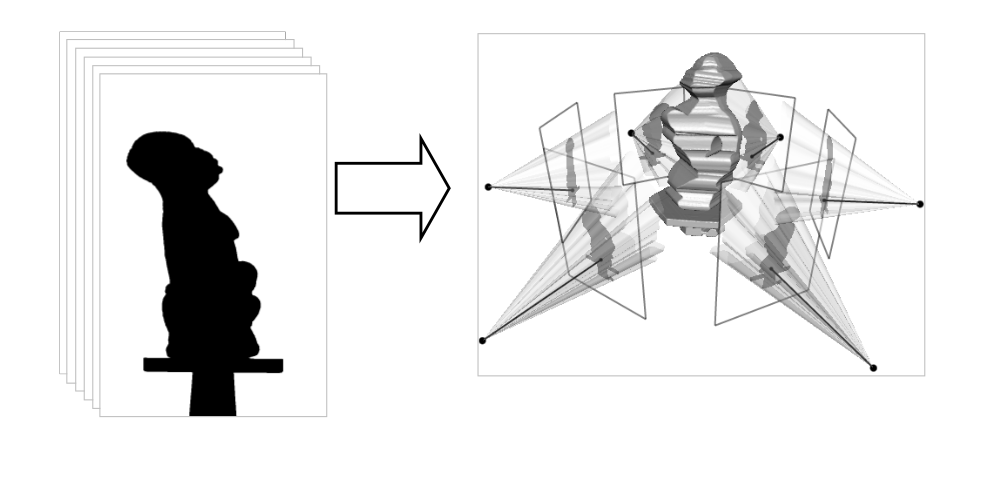
\includegraphics[width=1.0\textwidth]{img/carving6}
   \caption*{\tiny Source: How to prepare and deliver a presentation, by Roberto Cipolla [ppt]}
   \label{fig:carving6}
  \end{figure}
\end{frame}

%\begin{frame}
%  \centerline{\Huge BUT}
%\end{frame}
\begin{frame}
  \frametitle{Space Carving (silhouettes)}
  We get:
  \begin{itemize}
    \item Con\textbf{vex} hull
  \end{itemize}
  BUT:
  \begin{itemize}
    \item Finding silhouettes necessary (can use Green Screen)
    \item Often one (simple) object only
  \end{itemize}
\end{frame}


\subsection*{Multi-View Stereo}

\begin{frame}
  \frametitle{Multi-View Stereo}
  \begin{enumerate}
    \item Make depth maps (from image pairs)
    \item Merge them
  \end{enumerate}
\end{frame}

\begin{frame}
  \frametitle{Multi-View Stereo: Active lighting} % separate sensor
  \begin{enumerate}
    \item Actively light environment
    \item Find back light in image
    \item Estimate pixel depth
  \end{enumerate}
  Example: Kinect (structured light):
  \begin{figure}[htb!]
   \centering
   \subfigure{
    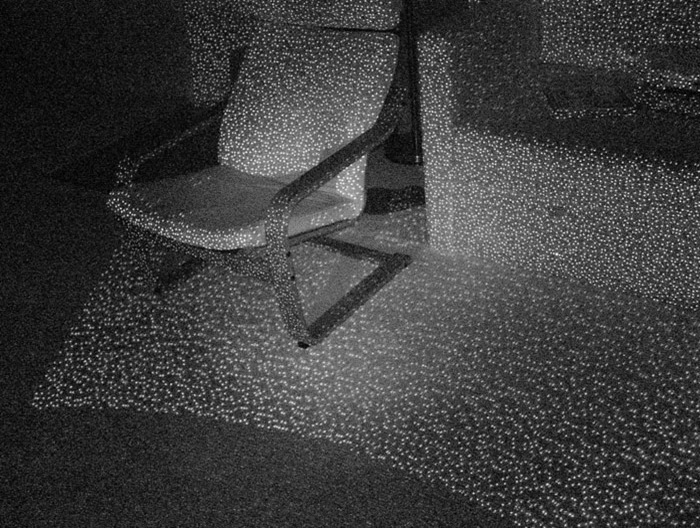
\includegraphics[width=0.4\textwidth]{img/kinect_pattern}  %\label{fig:}
   }
   \subfigure{
    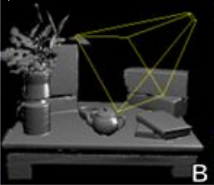
\includegraphics[width=0.4\textwidth]{img/kinect}  %\label{fig:}
   }
   \caption*{\tiny Left: http://www.hackengineer.com/structured-light-vs-microsoft-kinect  \\ Right: KinectFusion: Real-time 3D Reconstruction and Interaction Using a Moving Depth Camera (2011)}
  \end{figure}
\end{frame}

\begin{frame}
  \frametitle{Multi-View Stereo: Photo-Consistancy}
  For every pixel:
  \begin{enumerate}
    \item Find corresponding pixel in second image
    \item Estimate pixel depth
  \end{enumerate}

  \begin{figure}[htb!]
   \centering
   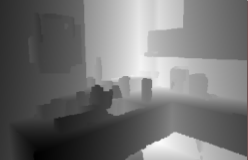
\includegraphics[width=0.3\textwidth]{img/depthmap_single}
   \caption*{\tiny Source: Manhattan-world Stereo [2009]}
  \end{figure}
  \begin{figure}[htb!]
   \centering
   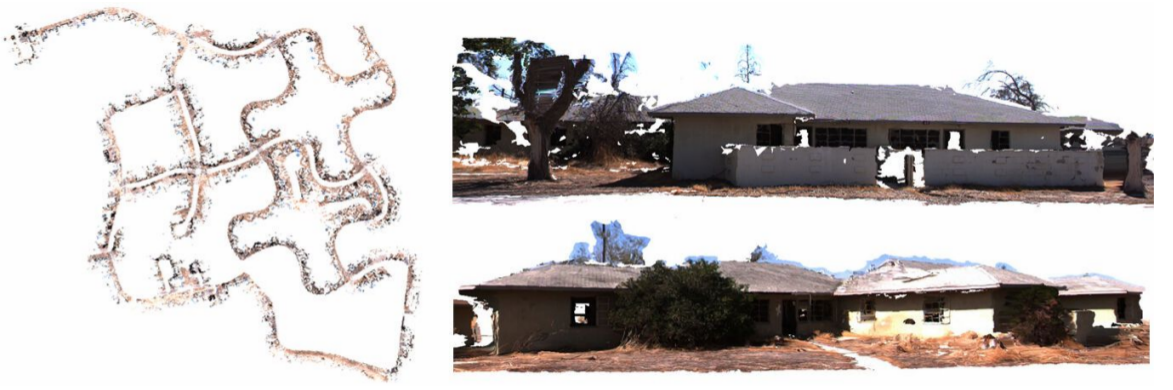
\includegraphics[width=0.8\textwidth]{img/depthmap_merged}
   \caption*{\tiny Source: Real-Time Visibility-Based Fusion of Depth Maps [2007]}
  \end{figure}
\end{frame}

%\begin{frame}
%  \centerline{\Huge BUT}
%\end{frame}
\begin{frame}
  \frametitle{Multi-View Stereo: Photo-Consistancy}
  BUT:
  \begin{itemize}
    \item Needs photo-consistancy measure \\
          (textured + lambertian objects)
  \end{itemize}
\end{frame}




\section{Method}

\begin{frame}
  \frametitle{Method}
    Find objects \emph{indirectly} by visibility and missing visibility (occlusion)
    \begin{itemize}
      \item Structure from Motion
      \item Space carving
      \item (Surface reconstruction + Texture Mapping)
    \end{itemize}
\end{frame}

\begin{frame}
  \frametitle{Method: Space Carving}
  We get this:
  \begin{figure}[htb!]
   \centering
   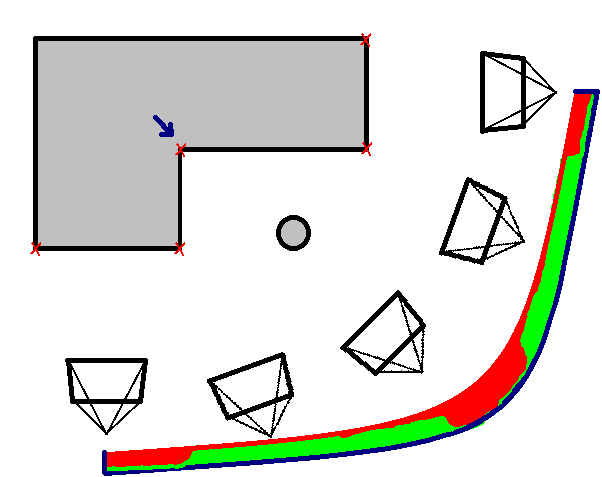
\includegraphics[width=0.8\textwidth]{img/visibilityocclusiontrack}
  \end{figure}
\end{frame}

\begin{frame}
  \frametitle{Method: Space Carving}
  We do this:
  \begin{figure}[htb!]
   \centering
   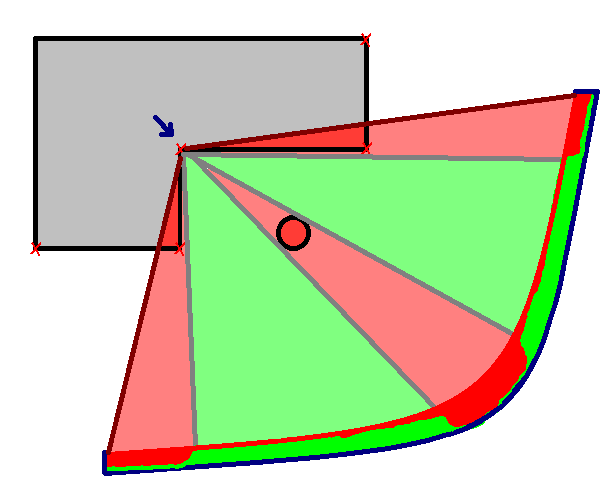
\includegraphics[width=0.8\textwidth]{img/visibilityocclusioncarving}
  \end{figure}
\end{frame}



\section{Results}

\begin{frame}
  \frametitle{Results}
  Shown for 3 examples:
  \begin{itemize}
    \item Image sequence
    \item Sparse point cloud (VisualSfM)
    \item Them: Multi-View Stereo CMVS/PMVS (2010)
    \item Our: Visibility-Occlusion Space Carving
  \end{itemize}
\end{frame}

\begin{frame}
  \frametitle{Result: car\_and\_wall1}
  \begin{figure}[htb!]
   \centering
   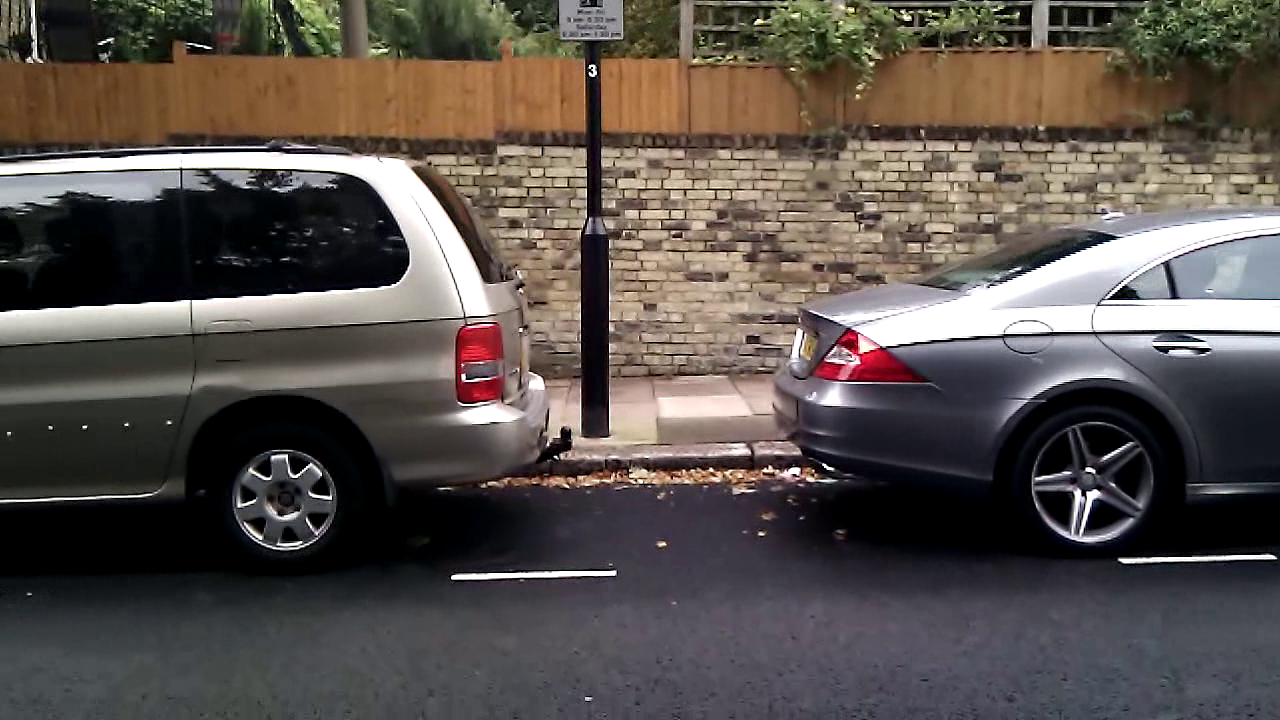
\includegraphics[width=0.9\textwidth]{img/car_and_wall1_frame}  %\label{fig:}
  \end{figure}
  \begin{itemize}
    \item \href{run:./vid/01-result1-seq.mp4}{\textbf{Image sequence}} \\
    \item \href{run:./vid/02-result1-sparse.mp4}{Sparse point cloud} \\
    \item \href{run:./vid/03-result1-mvs.mp4}{Multi-View Stereo (them)} \\
    \item \href{run:./vid/04-result1-visocc.mp4}{Visibility-Occlusion Space Carving (our)} \\
  \end{itemize}
\end{frame}
\begin{frame}
  \frametitle{Result: car\_and\_wall1}
  \begin{figure}[htb!]
   \centering
   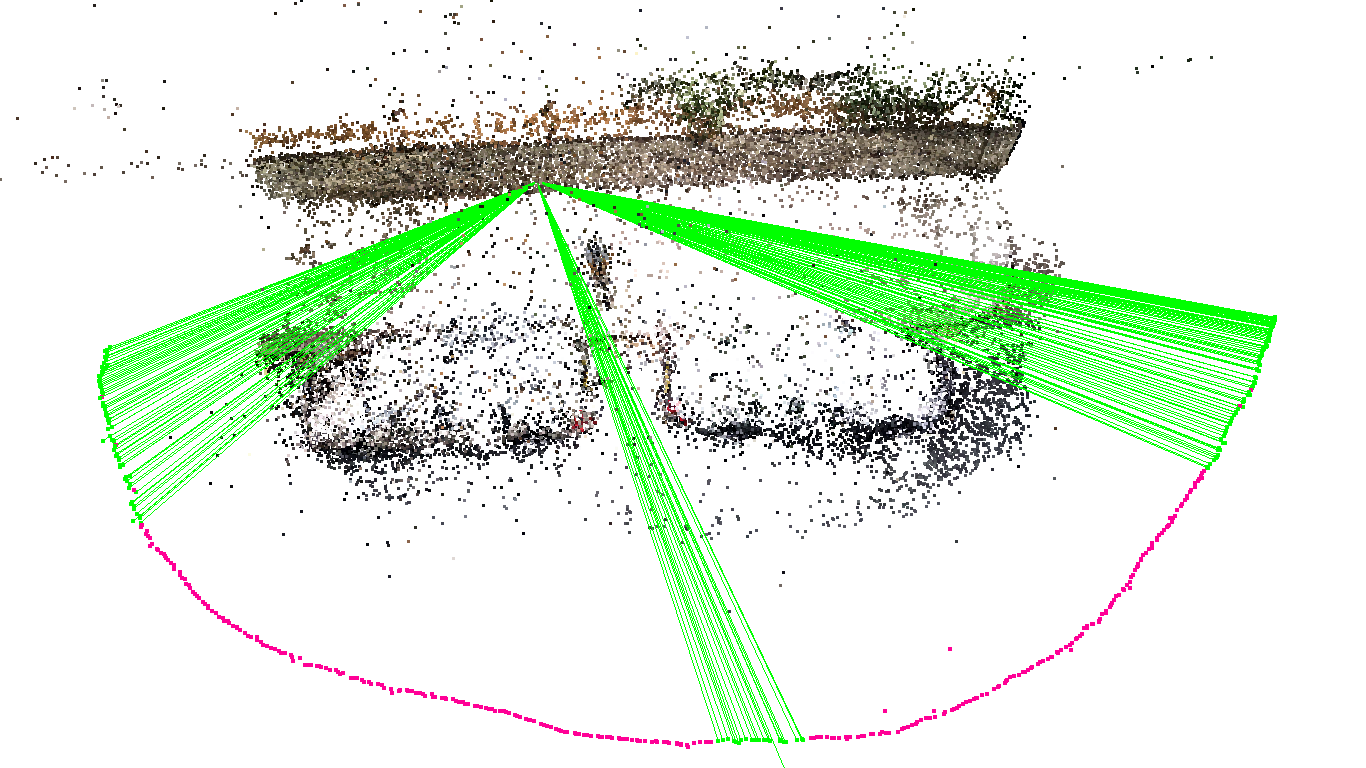
\includegraphics[width=0.9\textwidth]{img/car_and_wall1_sparse}  %\label{fig:}
  \end{figure}
  \begin{itemize}
    \item \href{run:./vid/01-result1-seq.mp4}{Image sequence} \\
    \item \href{run:./vid/02-result1-sparse.mp4}{\textbf{Sparse point cloud}} \\
    \item \href{run:./vid/03-result1-mvs.mp4}{Multi-View Stereo (them)} \\
    \item \href{run:./vid/04-result1-visocc.mp4}{Visibility-Occlusion Space Carving (our)} \\
  \end{itemize}
\end{frame}
\begin{frame}
  \frametitle{Result: car\_and\_wall1}
  \begin{figure}[htb!]
   \centering
   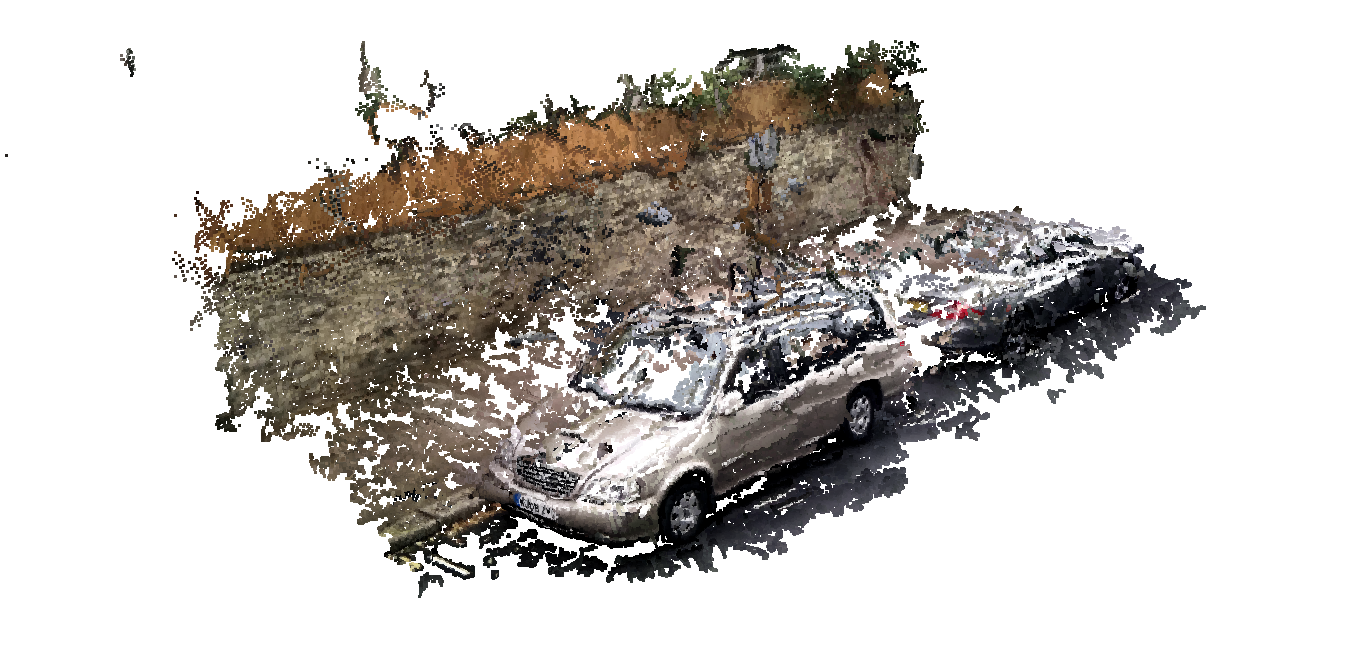
\includegraphics[width=0.9\textwidth]{img/car_and_wall1_dense}  %\label{fig:}
  \end{figure}
  \begin{itemize}
    \item \href{run:./vid/01-result1-seq.mp4}{Image sequence} \\
    \item \href{run:./vid/02-result1-sparse.mp4}{Sparse point cloud} \\
    \item \href{run:./vid/03-result1-mvs.mp4}{\textbf{Multi-View Stereo (them)}} \\
    \item \href{run:./vid/04-result1-visocc.mp4}{Visibility-Occlusion Space Carving (our)} \\
  \end{itemize}
\end{frame}
\begin{frame}
  \frametitle{Result: car\_and\_wall1}
  \begin{figure}[htb!]
   \centering
   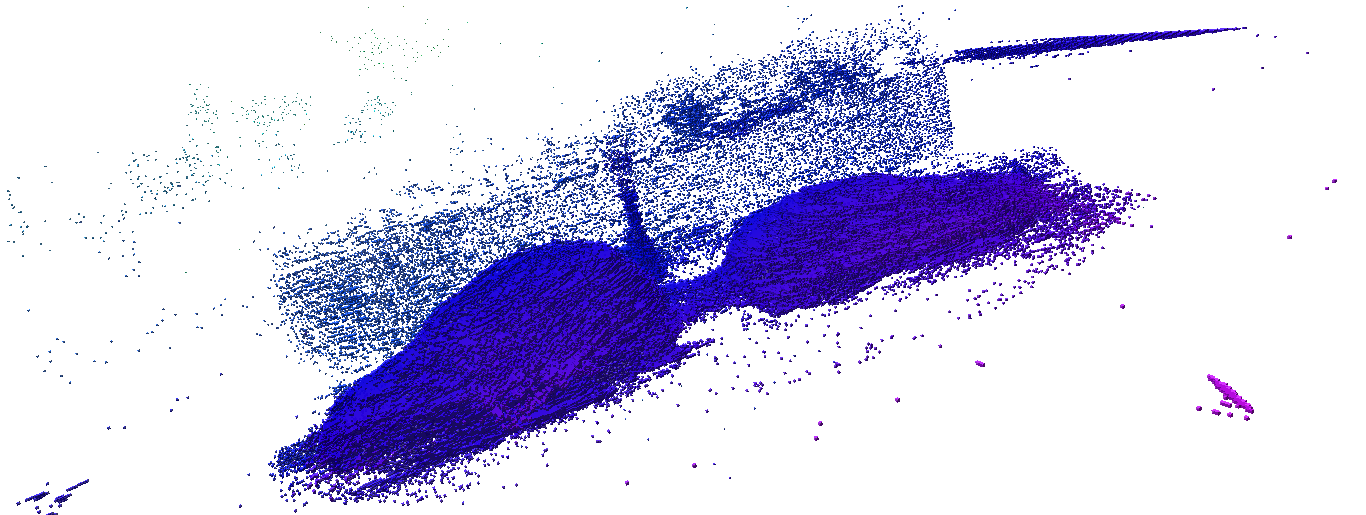
\includegraphics[width=0.9\textwidth]{img/car_and_wall1_carve2}  %\label{fig:}
  \end{figure}
  \begin{itemize}
    \item \href{run:./vid/01-result1-seq.mp4}{Image sequence} \\
    \item \href{run:./vid/02-result1-sparse.mp4}{Sparse point cloud} \\
    \item \href{run:./vid/03-result1-mvs.mp4}{Multi-View Stereo (them)} \\
    \item \href{run:./vid/04-result1-visocc.mp4}{\textbf{Visibility-Occlusion Space Carving (our)}} \\
  \end{itemize}
\end{frame}

\begin{frame}
  \frametitle{Result: sculpture1}
  \begin{figure}[htb!]
   \centering
   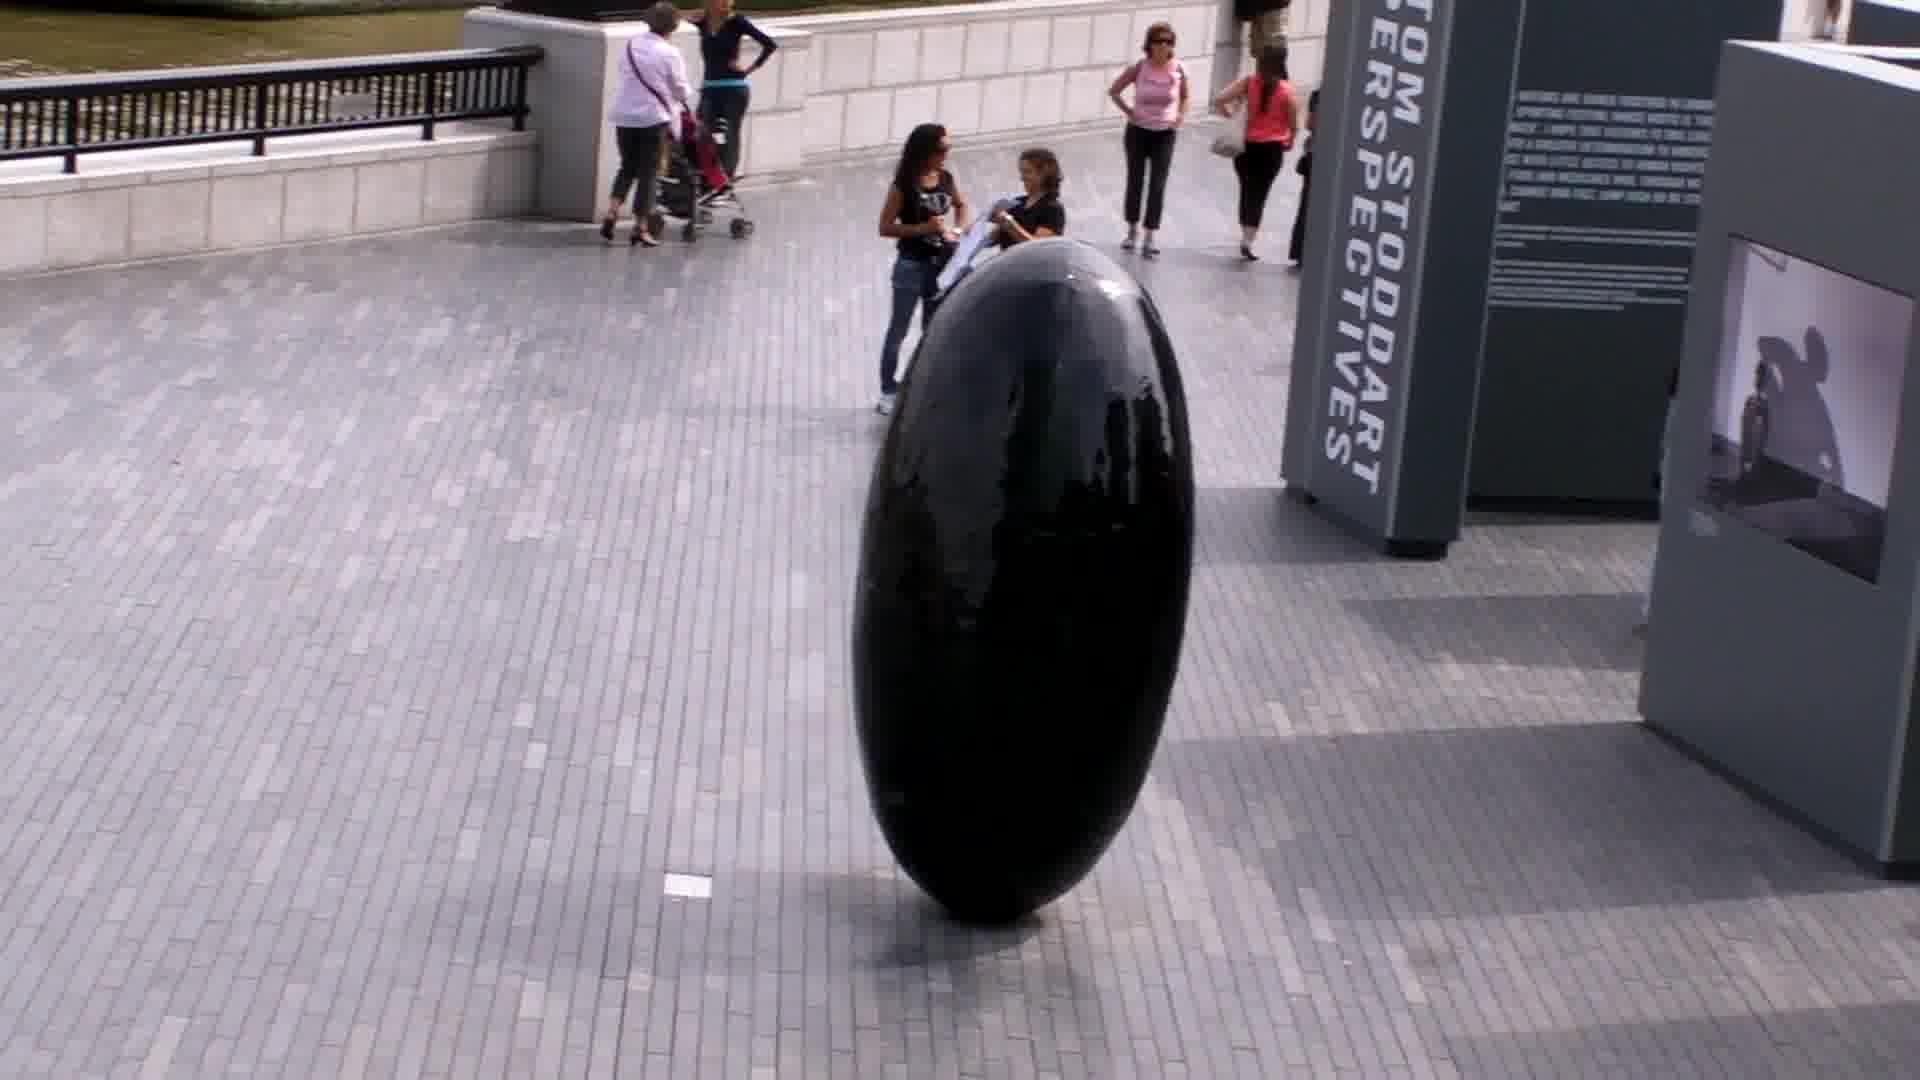
\includegraphics[width=0.9\textwidth]{img/sculpture1_frame}  %\label{fig:}
  \end{figure}
  \begin{itemize}
    \item \href{run:./vid/05-result2-seq.mp4}{\textbf{Image sequence}} \\
    \item \href{run:./vid/06-result2-sparse.mp4}{Sparse point cloud} \\
    \item \href{run:./vid/07-result2-mvs.mp4}{Multi-View Stereo (them)} \\
    \item \href{run:./vid/08-result2-visocc.mp4}{Visibility-Occlusion Space Carving (our)} \\
  \end{itemize}
\end{frame}
\begin{frame}
  \frametitle{Result: sculpture1}
  \begin{figure}[htb!]
   \centering
   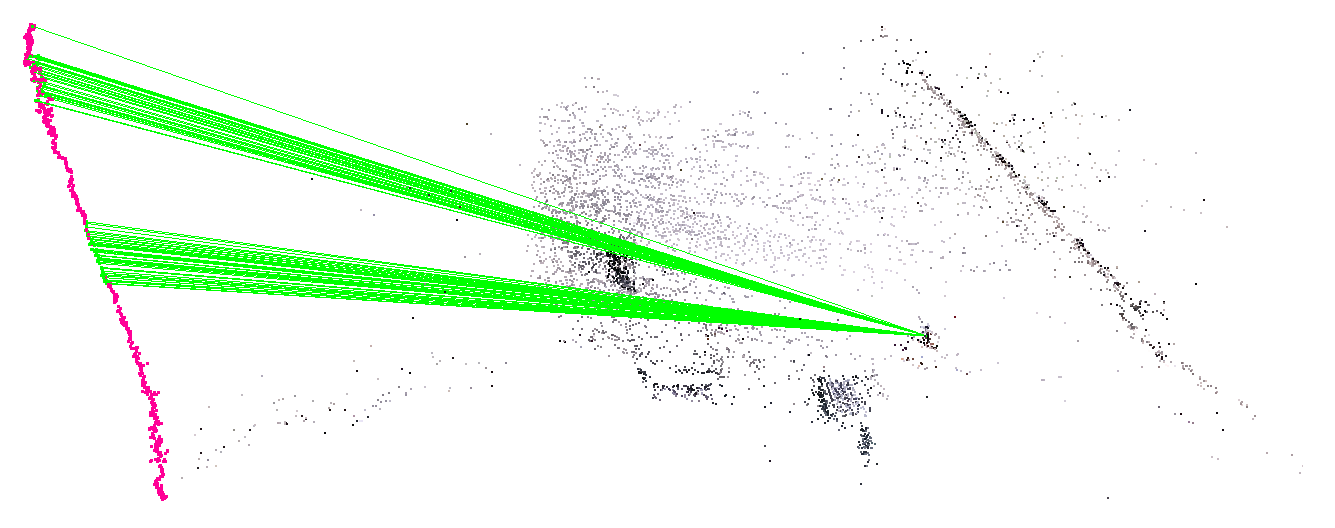
\includegraphics[width=0.9\textwidth]{img/sculpture1_sparse}  %\label{fig:}
  \end{figure}
  \begin{itemize}
    \item \href{run:./vid/05-result2-seq.mp4}{Image sequence} \\
    \item \href{run:./vid/06-result2-sparse.mp4}{\textbf{Sparse point cloud}} \\
    \item \href{run:./vid/07-result2-mvs.mp4}{Multi-View Stereo (them)} \\
    \item \href{run:./vid/08-result2-visocc.mp4}{Visibility-Occlusion Space Carving (our)} \\
  \end{itemize}
\end{frame}
\begin{frame}
  \frametitle{Result: sculpture1}
  \begin{figure}[htb!]
   \centering
   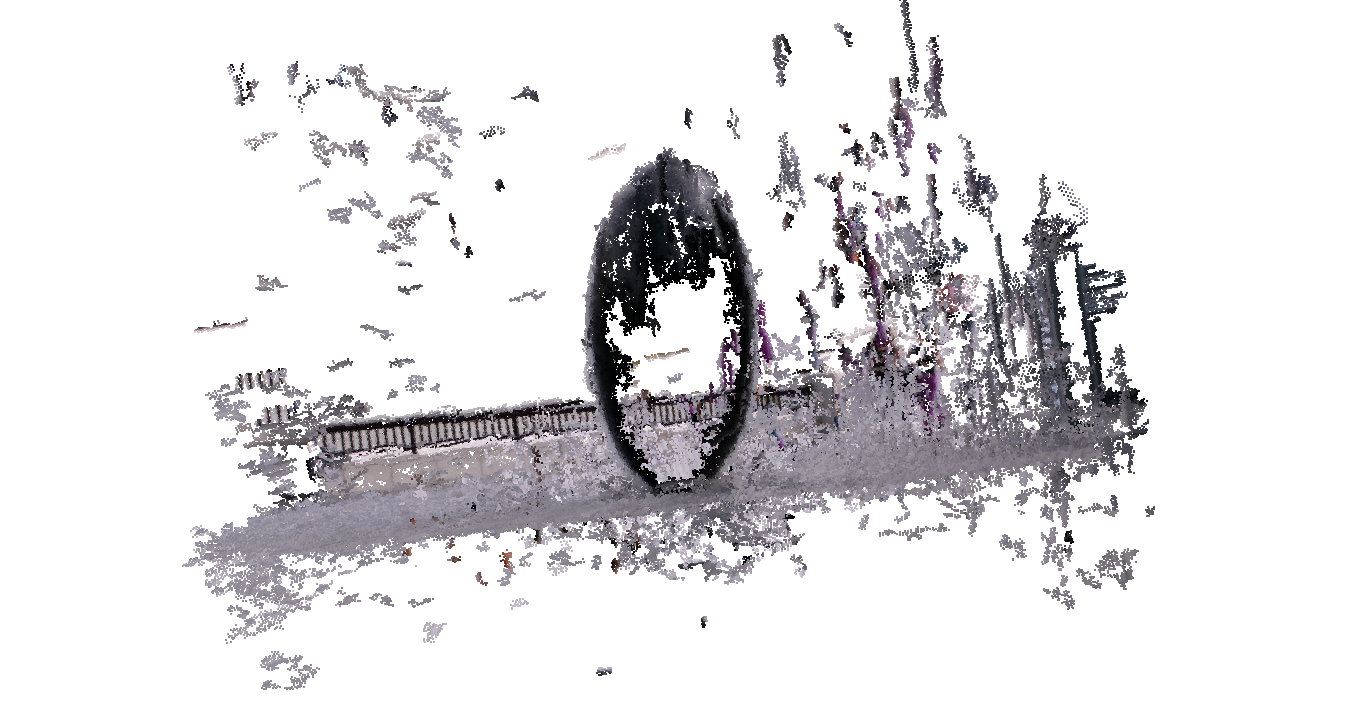
\includegraphics[width=0.9\textwidth]{img/sculpture1_dense}  %\label{fig:}
  \end{figure}
  \begin{itemize}
    \item \href{run:./vid/05-result2-seq.mp4}{Image sequence} \\
    \item \href{run:./vid/06-result2-sparse.mp4}{Sparse point cloud} \\
    \item \href{run:./vid/07-result2-mvs.mp4}{\textbf{Multi-View Stereo (them)}} \\
    \item \href{run:./vid/08-result2-visocc.mp4}{Visibility-Occlusion Space Carving (our)} \\
  \end{itemize}
\end{frame}
\begin{frame}
  \frametitle{Result: sculpture1}
  \begin{figure}[htb!]
   \centering
   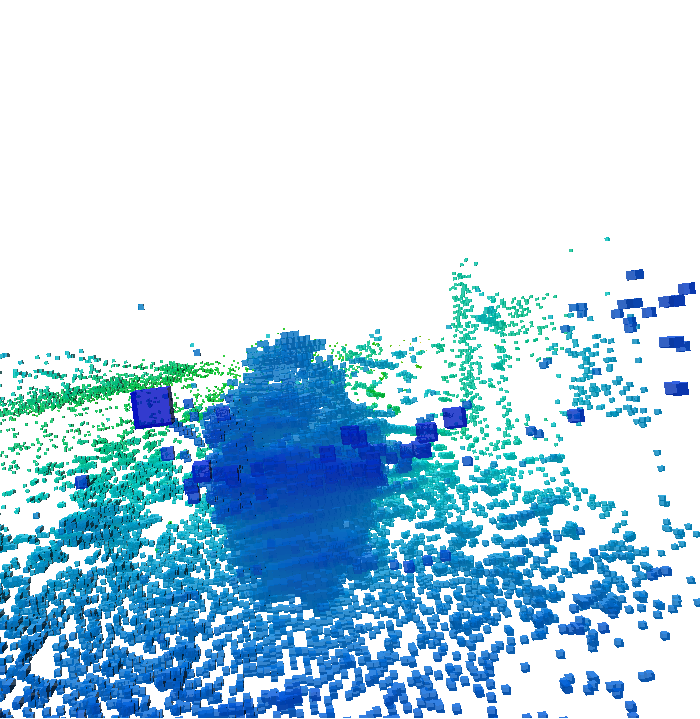
\includegraphics[width=0.4\textwidth]{img/sculpture1_carve2}  %\label{fig:}
  \end{figure}
  \begin{itemize}
    \item \href{run:./vid/05-result2-seq.mp4}{Image sequence} \\
    \item \href{run:./vid/06-result2-sparse.mp4}{Sparse point cloud} \\
    \item \href{run:./vid/07-result2-mvs.mp4}{Multi-View Stereo (them)} \\
    \item \href{run:./vid/08-result2-visocc.mp4}{\textbf{Visibility-Occlusion Space Carving (our)}} \\
  \end{itemize}
\end{frame}

\begin{frame}
  \frametitle{Result: memorial1}
  \begin{figure}[htb!]
   \centering
   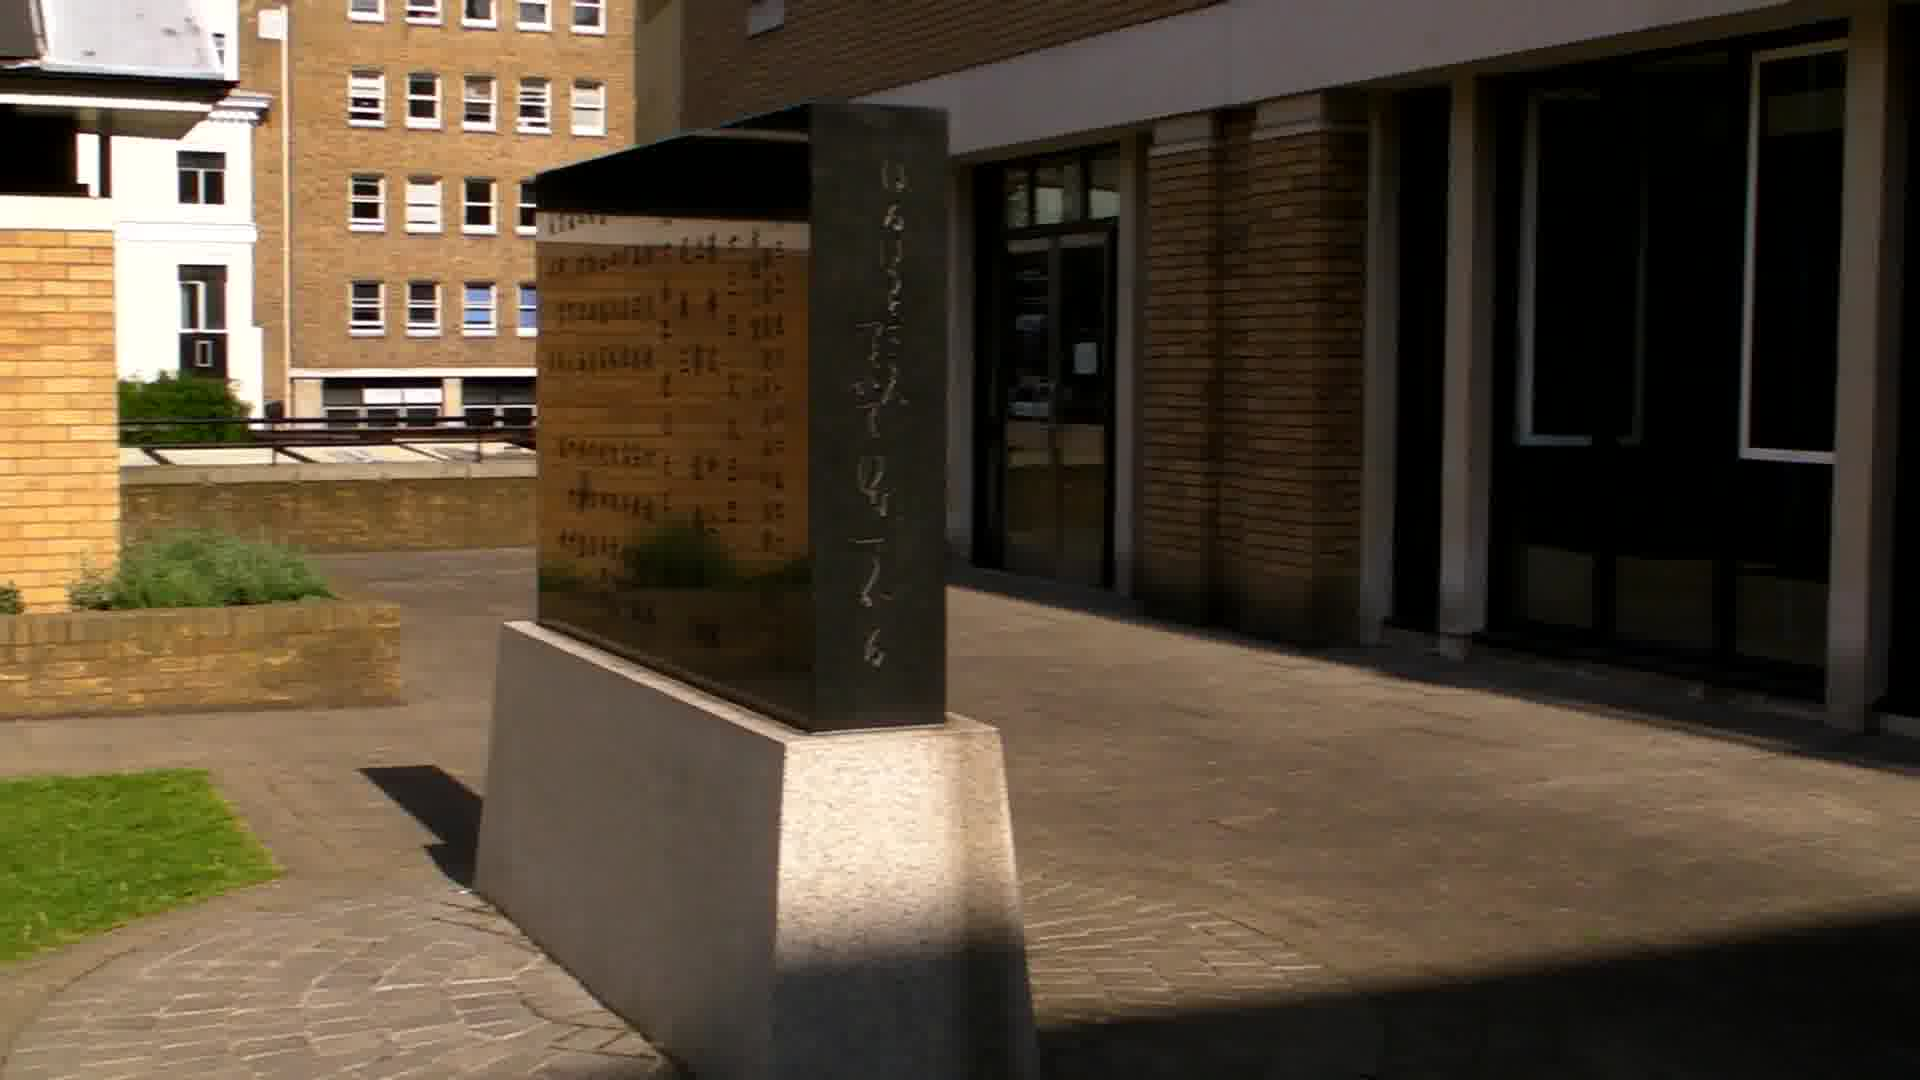
\includegraphics[width=0.9\textwidth]{img/memorial_frame}  %\label{fig:}
  \end{figure}
  \begin{itemize}
    \item \href{run:./vid/09-result3-seq.mp4}{\textbf{Image sequence}} \\
    \item \href{run:./vid/10-result3-sparse.mp4}{Sparse point cloud} \\
    \item \href{run:./vid/11-result3-mvs.mp4}{Multi-View Stereo (them)} \\
    \item \href{run:./vid/12-result3-visocc.mp4}{Visibility-Occlusion Space Carving (our)} \\
  \end{itemize}
\end{frame}
\begin{frame}
  \frametitle{Result: memorial1}
  \begin{figure}[htb!]
   \centering
   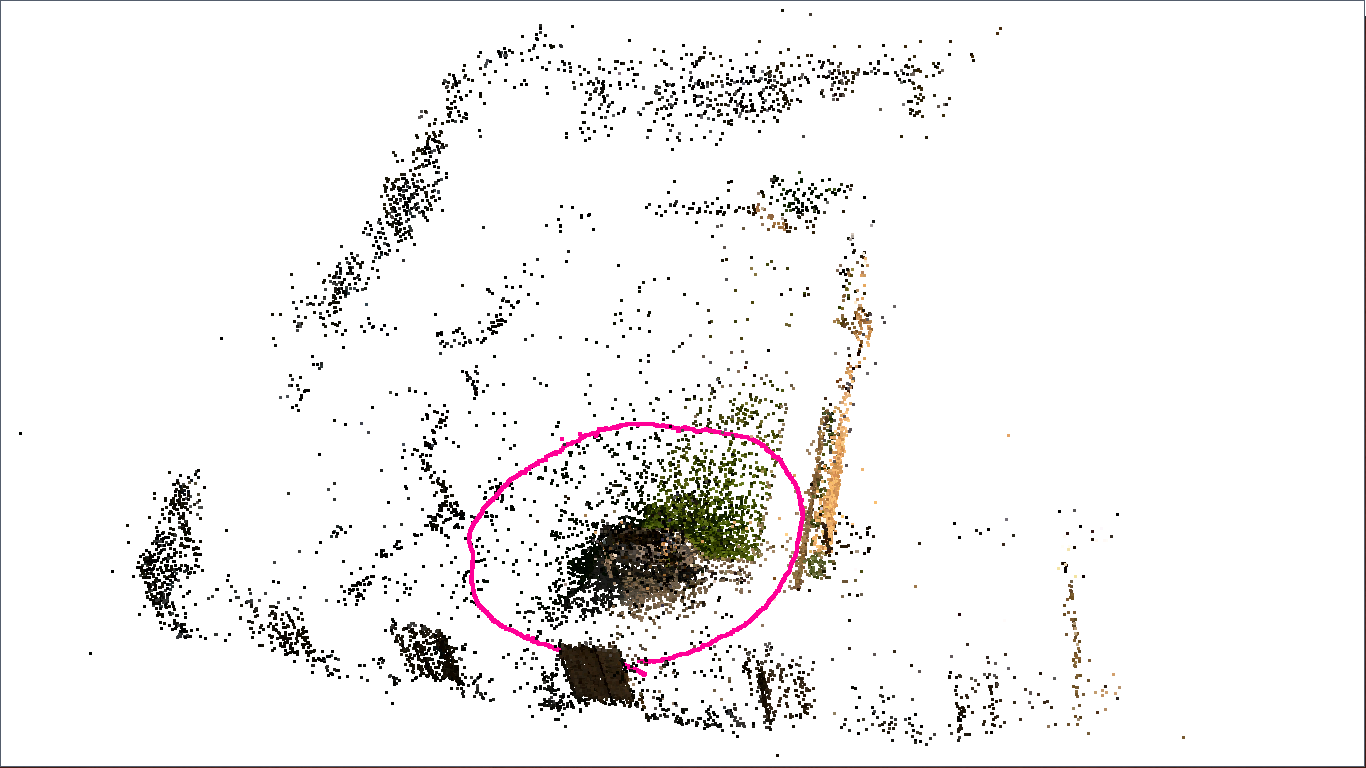
\includegraphics[width=0.9\textwidth]{img/memorial_sparse}  %\label{fig:}
  \end{figure}
  \begin{itemize}
    \item \href{run:./vid/09-result3-seq.mp4}{Image sequence} \\
    \item \href{run:./vid/10-result3-sparse.mp4}{\textbf{Sparse point cloud}} \\
    \item \href{run:./vid/11-result3-mvs.mp4}{Multi-View Stereo (them)} \\
    \item \href{run:./vid/12-result3-visocc.mp4}{Visibility-Occlusion Space Carving (our)} \\
  \end{itemize}
\end{frame}
\begin{frame}
  \frametitle{Result: memorial1}
  \begin{figure}[htb!]
   \centering
   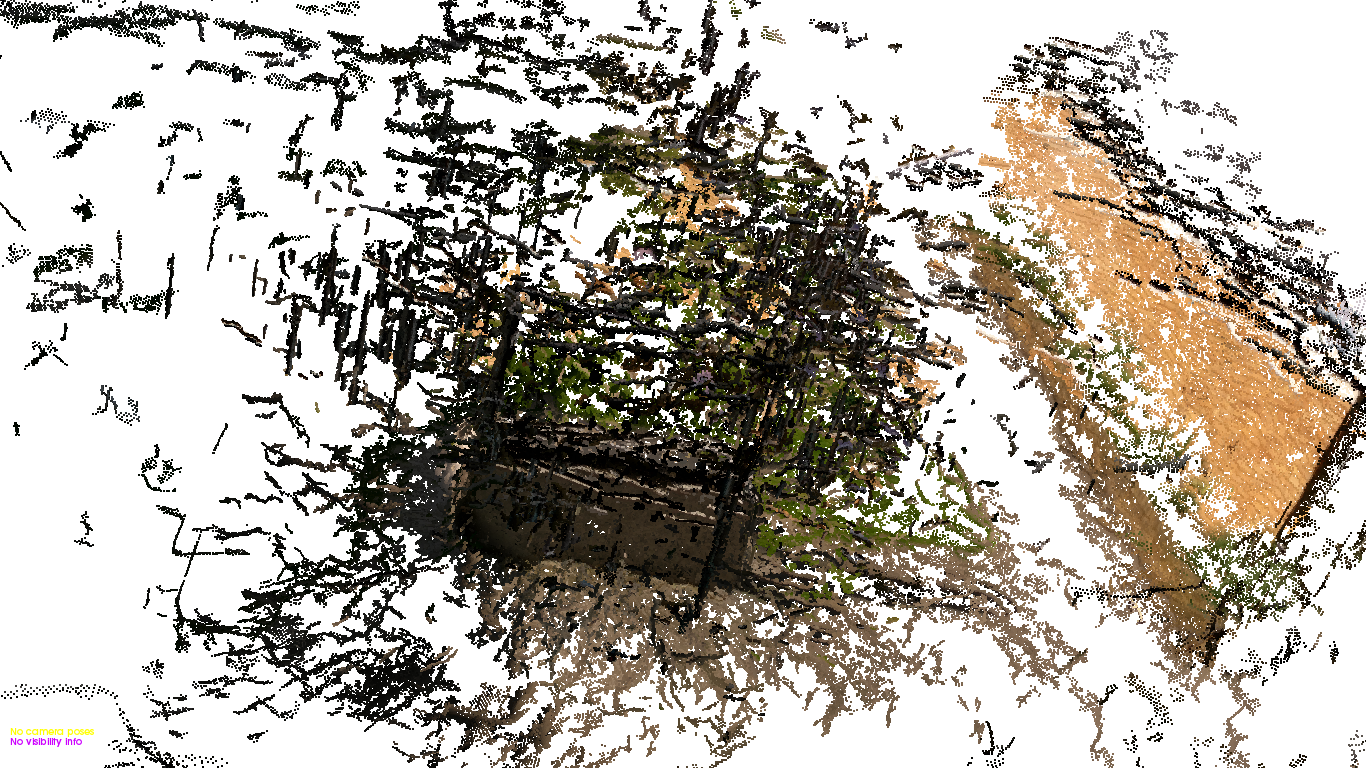
\includegraphics[width=0.9\textwidth]{img/memorial_dense}  %\label{fig:}
  \end{figure}
  \begin{itemize}
    \item \href{run:./vid/09-result3-seq.mp4}{Image sequence} \\
    \item \href{run:./vid/10-result3-sparse.mp4}{Sparse point cloud} \\
    \item \href{run:./vid/11-result3-mvs.mp4}{\textbf{Multi-View Stereo (them)}} \\
    \item \href{run:./vid/12-result3-visocc.mp4}{Visibility-Occlusion Space Carving (our)} \\
  \end{itemize}
\end{frame}
\begin{frame}
  \frametitle{Result: memorial1}
  \begin{figure}[htb!]
   \centering
   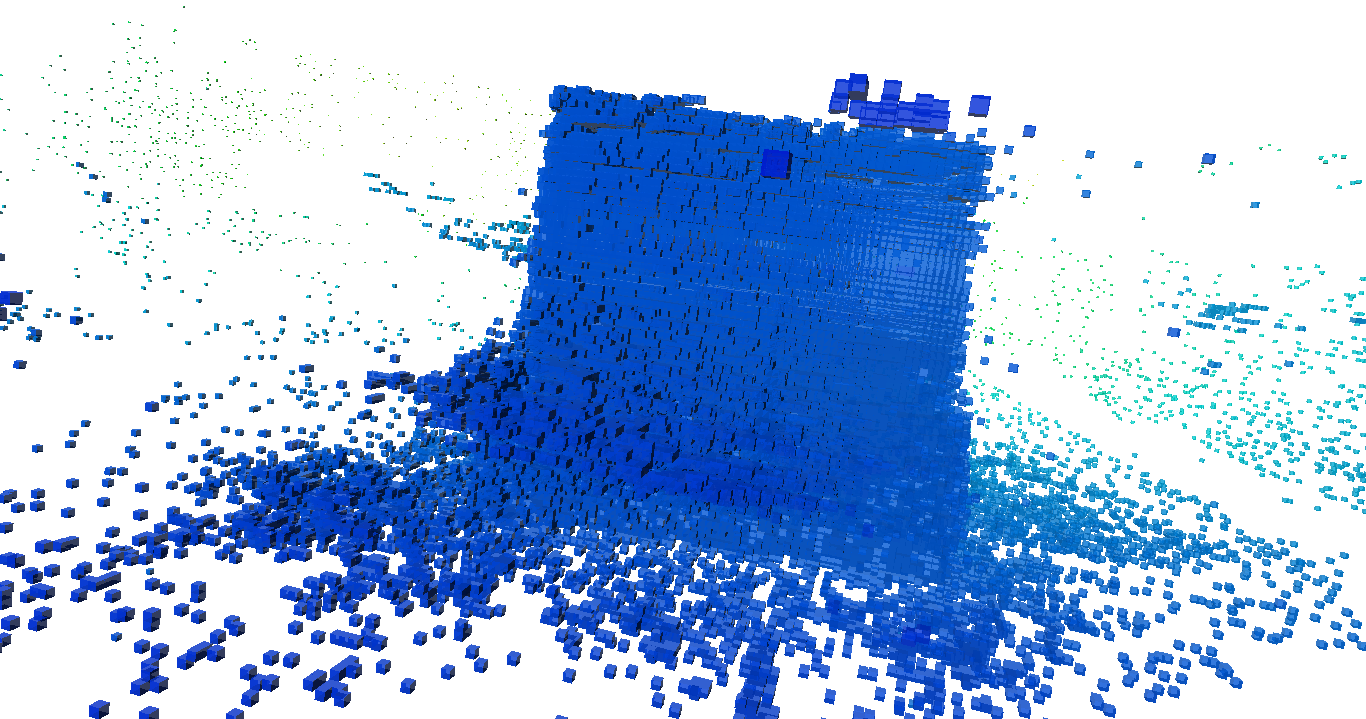
\includegraphics[width=0.9\textwidth]{img/memorial_carve2}  %\label{fig:}
  \end{figure}
  \begin{itemize}
    \item \href{run:./vid/09-result3-seq.mp4}{Image sequence} \\
    \item \href{run:./vid/10-result3-sparse.mp4}{Sparse point cloud} \\
    \item \href{run:./vid/11-result3-mvs.mp4}{Multi-View Stereo (them)} \\
    \item \href{run:./vid/12-result3-visocc.mp4}{\textbf{Visibility-Occlusion Space Carving (our)}} \\
  \end{itemize}
\end{frame}


\section{Conclusion}

\begin{frame}
  \frametitle{Conclusion}
  \begin{itemize}
    \item Needs enough data (view points)
    \item Needs textured background objects
    \item Can outperform state-of-the-art
  \end{itemize}
  \pause
  \begin{figure}[htb!]
   \centering
   \subfigure{
    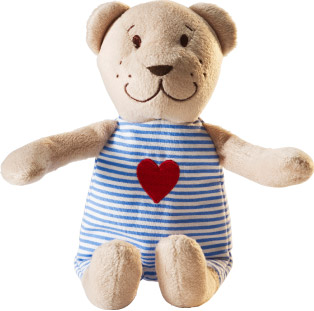
\includegraphics[width=0.3\textwidth]{img/bjorn_ikea}  %\label{fig:}
   }
   \subfigure{
    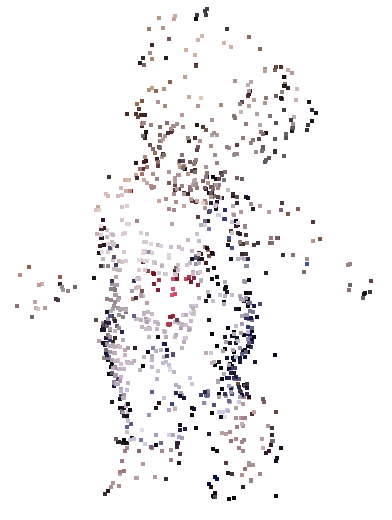
\includegraphics[width=0.3\textwidth]{img/bjorn}  %\label{fig:}
   }
   \caption*{\tiny Left: http://www.ikea.com; right: sparse point cloud}
   \label{fig:bjorn}
  \end{figure}
\end{frame}


\section*{Question Resources}

\begin{frame}
  \frametitle{Texture-rich object}
  \begin{figure}[htb!]
   \centering
   \subfigure{
    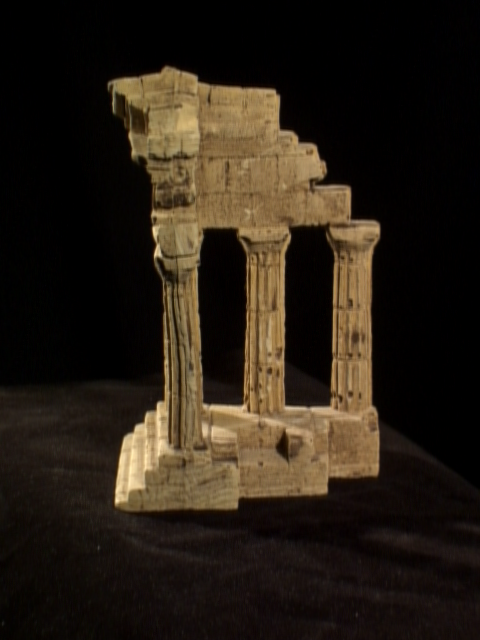
\includegraphics[width=0.45\textwidth]{img/temple_frame}  %\label{fig:}
   }
   \subfigure{
    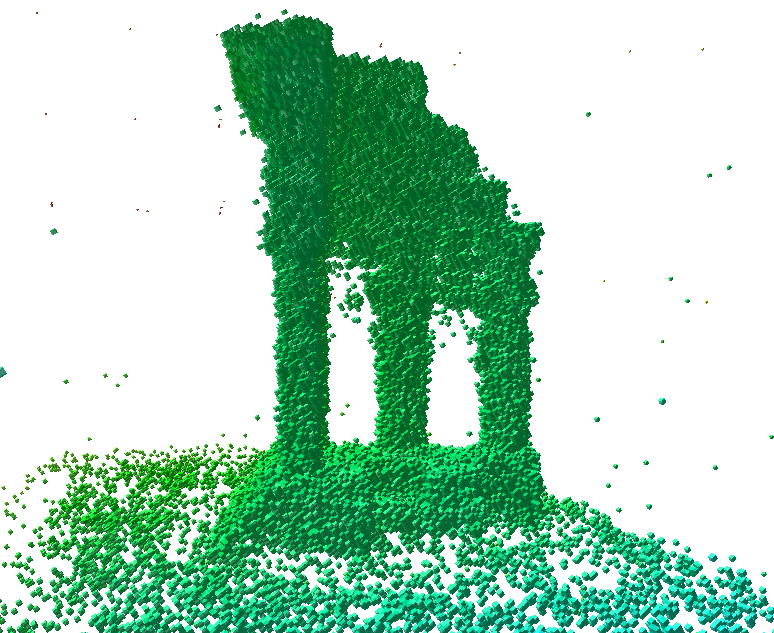
\includegraphics[width=0.45\textwidth]{img/temple_visocc}  %\label{fig:}
   }
   \caption*{\tiny Middelbury Multi-View Temple dataset (2006)}
  \end{figure}
  \href{run:./vid/13-temple-visocc.mp4}{\tiny Smoooooooth animation!} \\
\end{frame}

\begin{frame}
  \frametitle{`Bad' result}
  \begin{figure}[htb!]
   \centering
   \subfigure{
    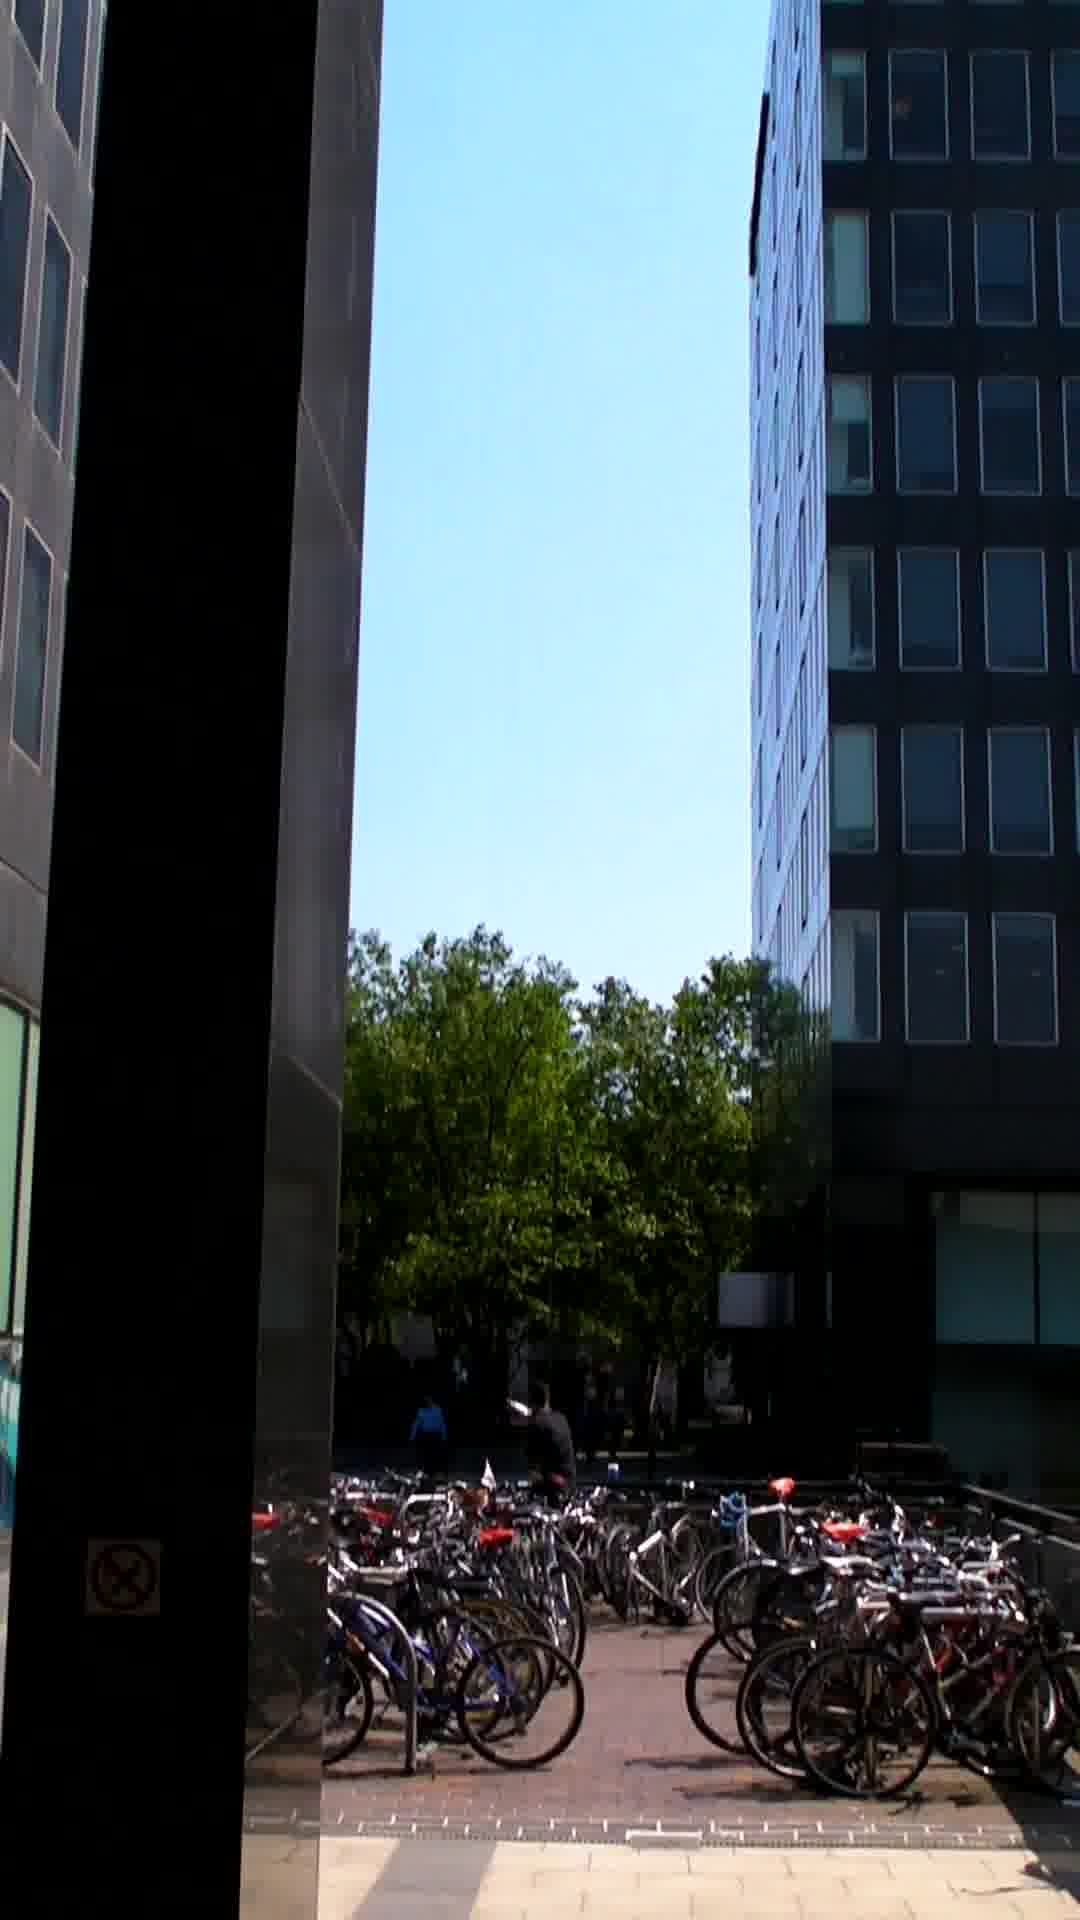
\includegraphics[width=0.25\textwidth]{img/failure_frame}  %\label{fig:}
   }
   \subfigure{
    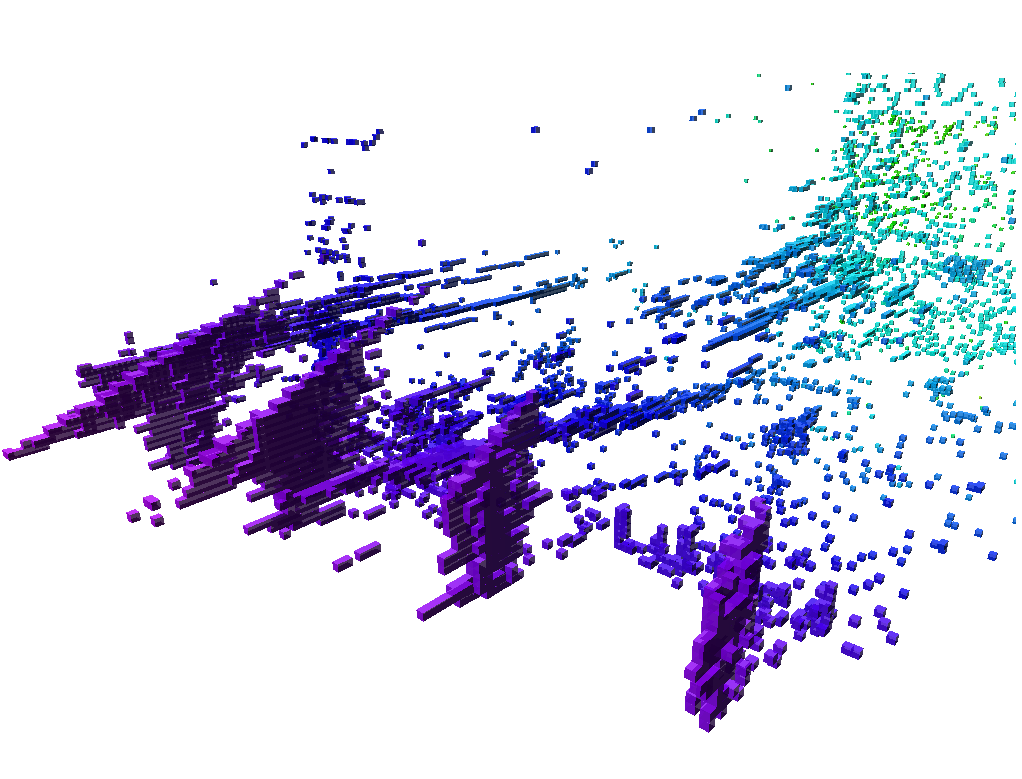
\includegraphics[width=0.7\textwidth]{img/failure_visocc}  %\label{fig:}
   }
  \end{figure}
\end{frame}

\begin{frame}
  \frametitle{Visibility-only Space Carving}
  \begin{figure}[htb!]
   \centering
   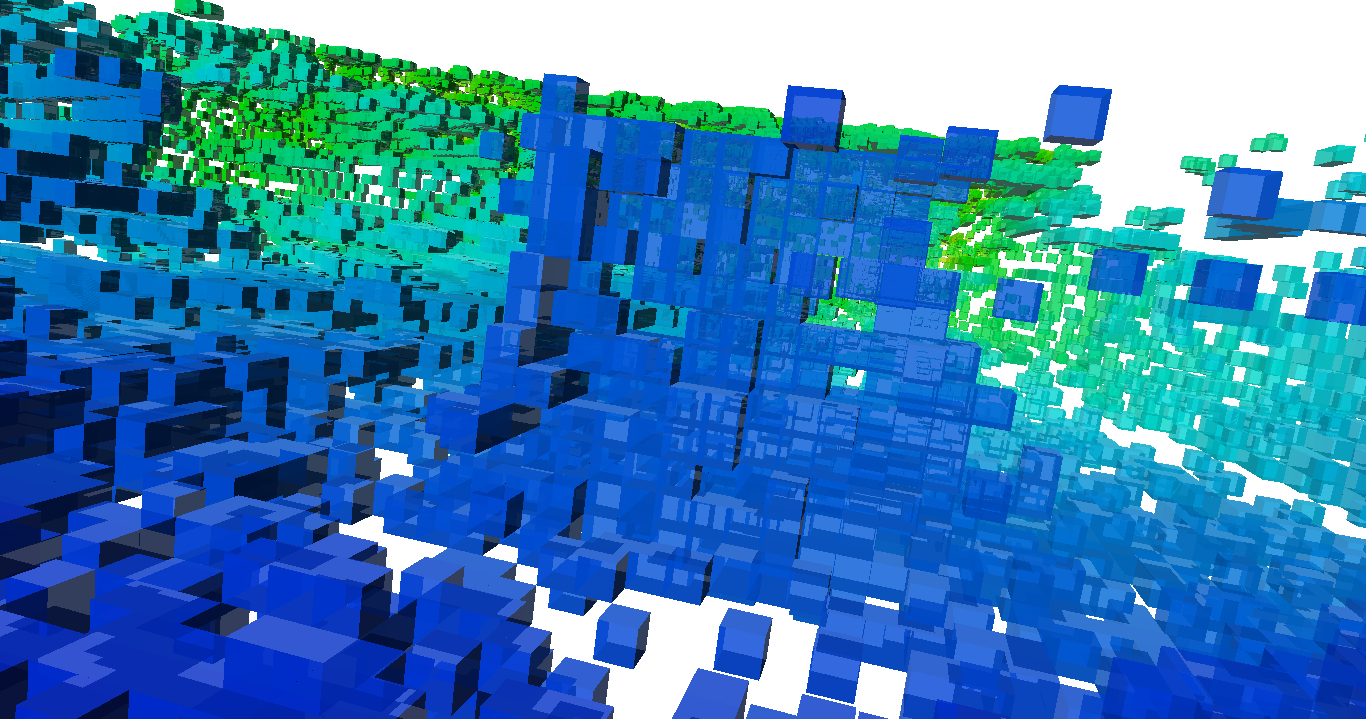
\includegraphics[width=0.8\textwidth]{img/memorial_carve1}
  \end{figure}
\end{frame}

\end{document}
